The Large Hadron Collider (LHC) is the world's largest and most powerful particle accelerator ever built whose sole purpose is to explore the fundamental interactions of nature. The LHC is located at the European Organization for Nuclear Research (CERN) in Geneva, situated right on the border of France and Switzerland.
The LHC is 27 km in circumference and can accelerate proton beams to a center of mass energy (\com{}) of 7 TeV each, resulting in a proton-proton collision with a \com{} of 14 TeV. For heavy-ion collisions each beam can also have a maximum \com{} of 7 TeV, with each nucleon having a maximum \com{} of about 5.5 TeV. Rather than a continuous beam of protons, protons are packed together in groups consisting of many billions of protons which is referred to as a proton bunch. The proton bunches are spaced apart from other proton bunches such that collisions happen at a set interval of every 25 nanoseconds. 
Likewise for heavy ion collisions, these particles are also grouped together in bunches, but have a different bunch spacing between them, ranging from 50 ns to 100 ns~\cite{Alice_first_pb_2023}. %For proton-proton collisions, LHC was designed to operate at a nominal luminosity of $\mathcal{L} = 10^{34} \mathrm{cm}^{-2}\mathrm{s}^{-1}$ but this has since been doubled to a sustained luminosity of $\mathcal{L} = 2 \times 10^{34} \mathrm{cm}^{-2}\mathrm{s}^{-1}$, while for heavy-ion collisions the maximum sustained luminosity is $\mathcal{L} = 10^{27} \mathrm{cm}^{-2}\mathrm{s}^{-1}$~\cite{ATLAS_run3_luminosity_and_detector}.

To accelerate protons to the desirable center of mass energies, a complex accelerator chain is used to accelerate protons in phases. The start of the accelerator chain is a linear accelerator, Linac4~\cite{linac4_yellow_report}, which accelerates protons to a \com{} of 160 MeV. This detector is relatively new having only been added during the long shutdown after Run 2 data taking, and replaces the previously used Linac2, which was only able to accelerate protons to a \com{} of 50 MeV. From Linac4, the protons are passed into the Proton Synchrotron Booster (PSB), which also underwent several upgrades of its own during the Run 2 long shutdown~\cite{psb_ls2_upgrade}, and is the first synchrotron in the accelerator chain. 
The PSB accelerates protons from 160 MeV to 2 GeV, before passing the protons along to the Proton Synchrotron (PS), which accelerates protons to 26 GeV. This part of the accelerator chain is essential as the proton bunches are compressed, split, and placed into the 25 ns spacing that the LHC requires. From here, and while keeping the established structure of the bunches, the bunches are passed into the Super Proton Synchrotron (SPS) which is the last step of the accelerator chain before the LHC\@. Here, the proton bunches are accelerated up to 450 GeV and passed either clockwise, or counter-clockwise, into the LHC where they are accelerated to their desired center of mass energies. This accelerator chain is depicted in Figure~\ref{fig:lhc_accelerator_chain}.

\begin{figure}[pht]
    \centering
    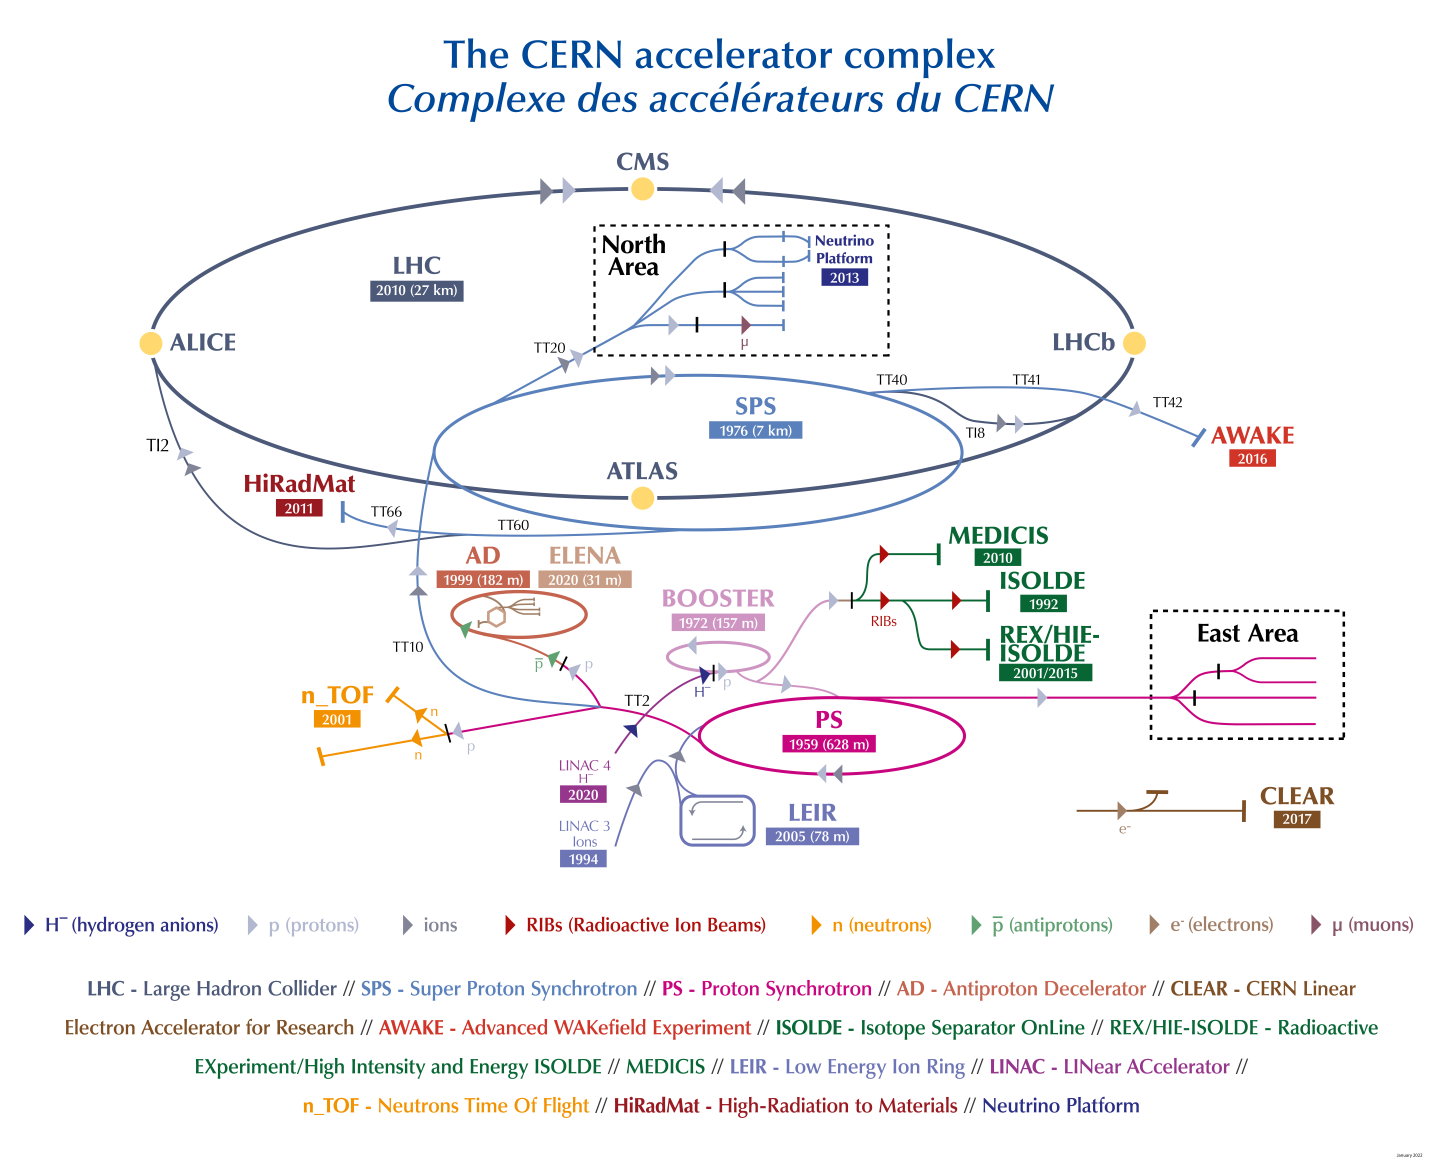
\includegraphics[width=0.7\textwidth]{figures/atlas/lhc_accelerator_chain.png}
    \caption{Shown are both the proton and heavy-ion accelerator chains. The proton accelerator chain starts from Linac4, goes to the PSB, then the PS and finally the SPS before being passed to the LHC\@. Heavy-ions follow a similar chain except their starting point is Linac3 and are then passed directly to the PS\@. Taken from~\cite{lhc_accelerator_chain_diagram}}\label{fig:lhc_accelerator_chain}
\end{figure}

At the LHC there are four main experiments. The two largest experiments, ATLAS~\cite{atlas_collaboration_paper} and CMS~\cite{cms_collaboration_paper}, are general, multi-purpose detectors designed to study a large range of topics in HEP, including precision measurements, searches for new physics, and even quark-gluon plasma from the heavy-ion collisions. There also exist two other experiments at the LHC with a more narrowed focus on their research activities. LHCb~\cite{lhcb_collaboration_paper} is a dedicated heavy-flavour physics experiment whose main goal is to search for new physics in CP violation, and rare decays of beauty and charm quarks. The ALICE~\cite{alice_collaboration_paper} experiment on the other hand is focused on heavy-ion collisions, more specifically the study of quark-gluon plasma that is produced during heavy-ion collisions. 

For Run 3, the LHC will operate at a \com{} collision energy of 13.6 TeV, and will take data from 2022--2026. The results covered in this thesis will be from the 2022 and 2023 data taking periods during Run 3.